\chapter{Internal Electrodes}
\subsection{The effects and uses of internal electrodes on 3D EIT image reconstructions}

\subsubsection{Motivation}
One of the shortcomings of EIT is low sensitivity away from the electrodes. 
For continuous monitoring of cardiac-related events an EIT protocol with an improved sensitivity 
near the heart and innermost regions of the lings may improve results and imaging accuracy.

\subsubsection{Problem}
EIT has low sensitivity away from the electrodes which are typically placed on the body surface. 
This chapter will investigate the use and application of internal electrodes and quantify the improvement 
in sensitivity and image reconstruction accuracy in simulation.

\subsubsection{Summary}
This chapter provides proof of principle of internal electrode configurations to 
improve EIT sensitivity and reconstruction accuracy.
The goal of this chapter is to determine the viability of internal electrode use through a series of simulations and phantom measurements then validate
the imaging ability using one or two animals. 

We expect to show that using internal electrodes increases the sensitivity of the measurements to internal impedance changes 
and enables a higher resolution of image reconstructions in these central regions of the thorax. 

\subsubsection{Simulations}
To analyze the sensitivity changes due to different electrode 
configurations finite element models (FEMs) of a cylindrical tank were 
created with each of the tested electrode configurations. Figure~\ref{fig:tank_FEM} shows the four 
different configurations that were tested: a 2D 
electrode ring of 32 electrodes; a 3D configuration of 2 layers of 16 
electrodes (3D(a)); a second 3D configuration of 2 layers of 15 electrodes 
plus 2 central internal electrodes inline with the electrode planes (3D(b)); and a final 3D configuration of 
2 layers of 14 electrodes with 4 central internal electrodes evenly spaced between the electrode planes (3D(c)).

\begin{figure}[!ht]
\centering
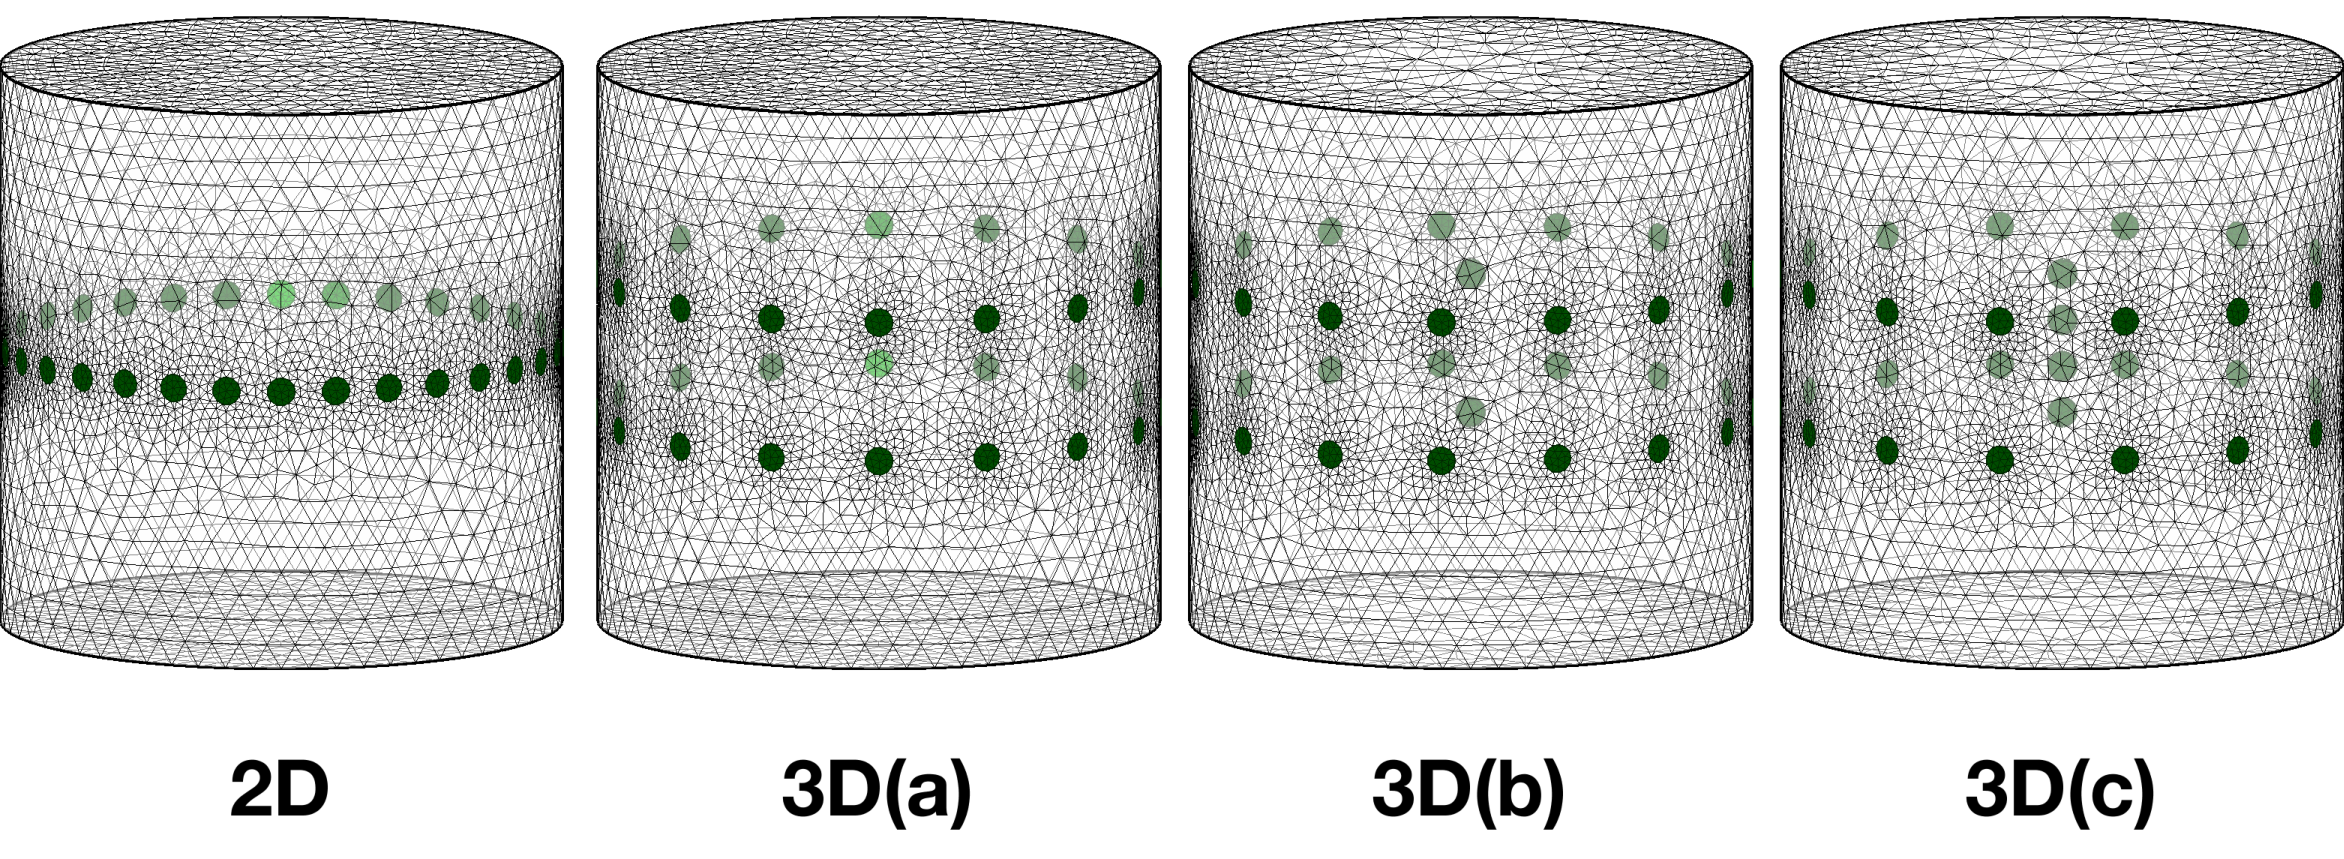
\includegraphics[width=\textwidth]{chapter_5/imgs/FEM_Comparison.pdf}
\caption[Internal electrode configurations]{4 configurations of electrodes were tested: 2D) a single ring of 32 electrodes; 
	3D(a) 2 rows of 16 external electrodes; 3D(b) 2 rows of 15 external electrodes with 2 internal electrodes; and 3D(c) 2 rows 
of 14 external electrodes and 4 internal electrodes.}
\label{fig:tank_FEM}
\end{figure}

The tank in the simulations has a height of 2 m, radius of 1 m, and the electrode radius
is 0.05 m for both the round external electrodes and the spherical internal electrodes.
In the 3D configurations the plane separation is 0.5 m and in all configurations the radial
spacing between electrodes is equal.
The background conductivity of the tank was 1 S/m and the conductivity of the target was
10 S/m.

When reconstructing images a conductive target was added to the tank
centred at a height of 1 m at the midpoint of the tank radius. The target
object radius is 0.4 m.

The reconstructions of the conductive object with and without additive noise are shown in Figure~\ref{fig:reconstruction_comparison}.
To generate EIT images from voltage measurements, the 3D GREIT
reconstruction algorithm
was used~\parencite{Adler2009}. A spherical
conductive target with a radius of 20\% of the tank radius
was placed midway between the centre and boundary
of the tank, in a region with typically low sensitivity.
The inverse problem hyperparameter
was selected so that in all instances the amount of measurement
noise that propagated from the measurements into the final images
was equal.

Preliminary reconstructions on simulated data show that internal electrodes are able to reconstruct a conductive object closer to its true 
size based on visual inspection, but more simulations are required to quantify the improvements. These preliminary reconstructions are shown in
Figure~\ref{fig:reconstruction_comparison}. The top row shows reconstructions with no additive noise, and the second row shows reconstructions on measurements with 5dB of 
additive noise.

\begin{figure}[!ht]
\centering
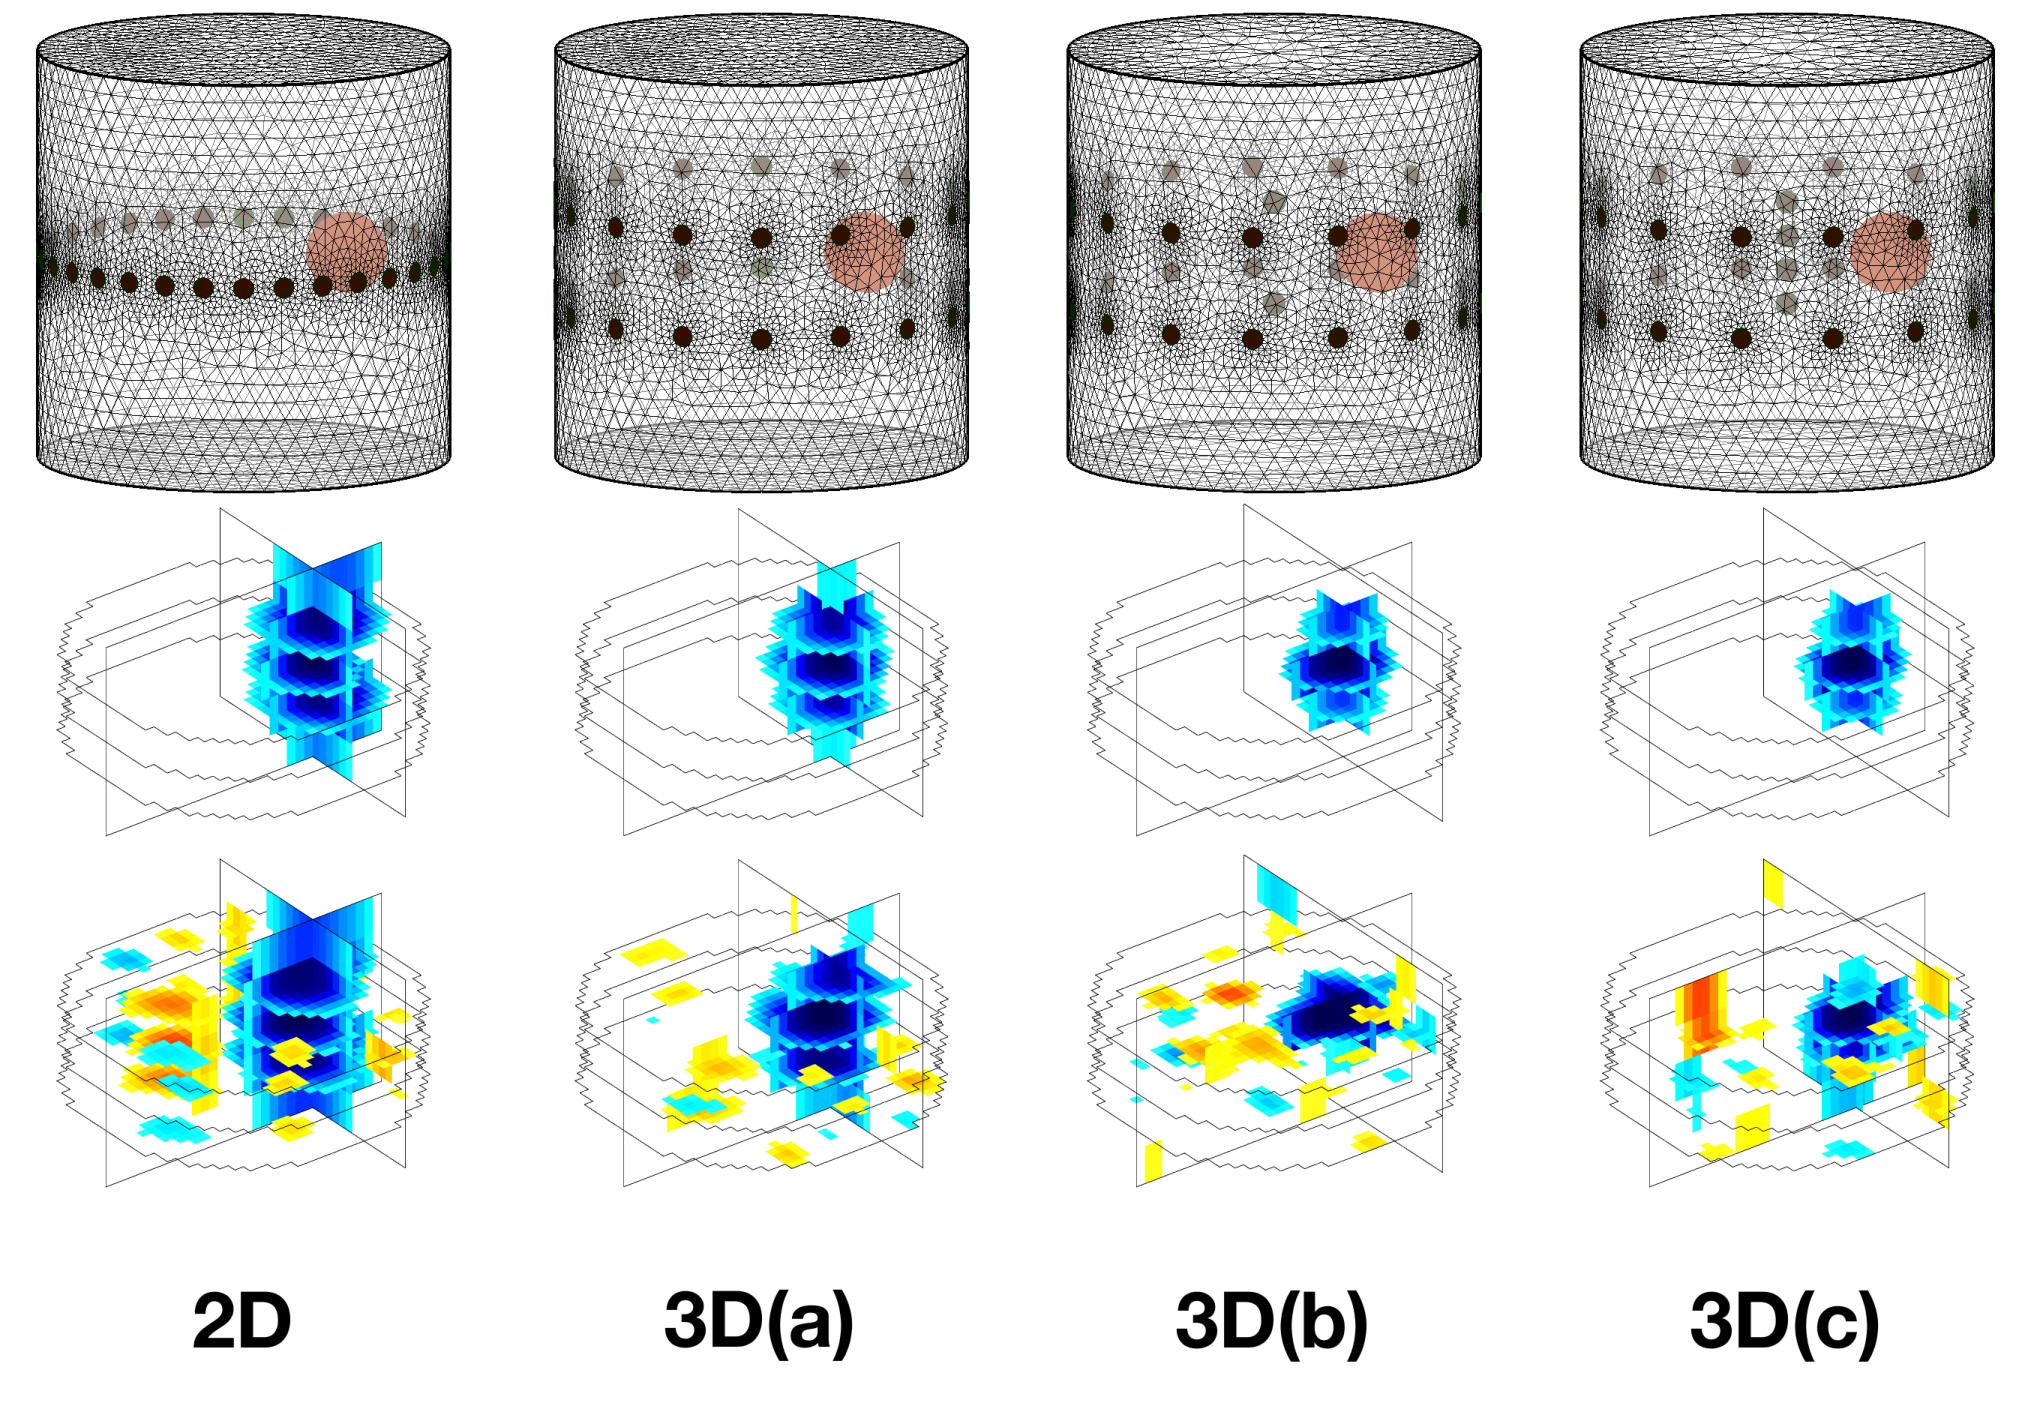
\includegraphics[width=\textwidth]{chapter_5/imgs/Image_Comparison.pdf}
\caption[Internal electrode simulation reconstructions]{The top row shows reconstructions with no additive noise, and the second row shows reconstructions on measurements with 5dB of
additive noise.}
\label{fig:reconstruction_comparison}
\end{figure}

Preliminary results shown in Figure~\ref{fig:internal_sensitivity} show internal sensitivity distribution changes when using 2 and 4 internal electrodes compared to the
typical 2D and 3D configurations with only external electrodes. 


\begin{figure}[!ht]
\centering
%\includegraphics[trim=0 65 0 400,clip,width=\textwidth]{chapter2/imgs/Sensitivity_Comparison_new.pdf}
\includegraphics[width=\textwidth]{chapter_5/imgs/Sensitivity_Comparison_new.pdf}
\caption[Sensitivity with different internal electrode configurations]{Sensitivity distributions for electrode patterns from left to right: A single 2D electrode plane; 2 electrode planes of 16 electrodes 
each; 2 internal electrodes and 2 external electrode rings of 15 electrodes; 4 internal electrodes arranged between 2 planes of 14 external
electrodes}
\label{fig:internal_sensitivity}
\end{figure}

The sensitivity is then calculated from the jacobian ($J$)of  the reconstruction matrix as:
% Sens = log(sqrt(sum(J.^2))'./get_elem_volume(fmdl_3dc));
$$ S = \frac{\sqrt{\sum_{i}\vec{J}_{ij}^2}}{V_i}  $$
where $V_i$ is the volume of each respective voxel. 

These results show the expected increased sensitivity in the central regions of the model. To further improve internal sensitivity a new
measurement pattern is proposed that uses more measurements between the internal probe and peripheral electrodes. The proposed injection and measurement
pattern is shown in Figure~\ref{fig:modified_measurement}.
The sensitivity of the proposed pattern was compared to the sensitivity profile of the same configuration using 
the basic ``skip 4'' injection and measurement pattern which has been found to 
give good sensitivity in 2D and 3D external electrode configurations~\cite{Grychtol2016}.

\begin{figure}[!ht]
\centering
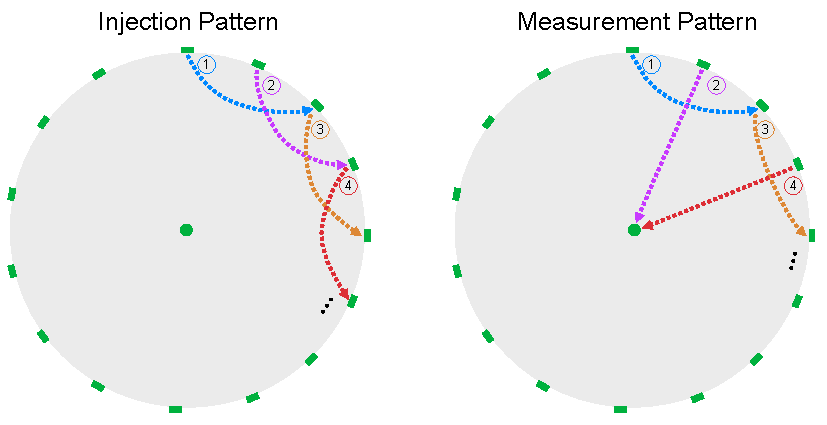
\includegraphics[width=\textwidth]{chapter_5/imgs/current_injection.pdf}
\caption[Current injection patterns with internal electrodes]{A proposed current injection and measurement pattern for \acrshort{eit} imaging with 2 internal electrodes.
The injection pattern is a typical ``skip 4 '' pattern injecting between every 5\textsuperscript{th} electrode in a square electrode layout and the
measurement pattern replaces every 2\textsuperscript{nd} measurement in the typical method with a measurement between the internal probe and
external rings. Note: this figure does not differentiate between upper and lower electrode planes, but all injections and measurements are done between 
the 2 planes.}
\label{fig:modified_measurement}
\end{figure}

Using this injection pattern preliminary results show a further increase in sensitivity in the internal regions without increasing the measurement
acquisition time. The sensitivity distribution for the new injection pattern is pictured in Figure~\ref{fig:modified_measurement_sens}.

\begin{figure}[!ht]
\centering
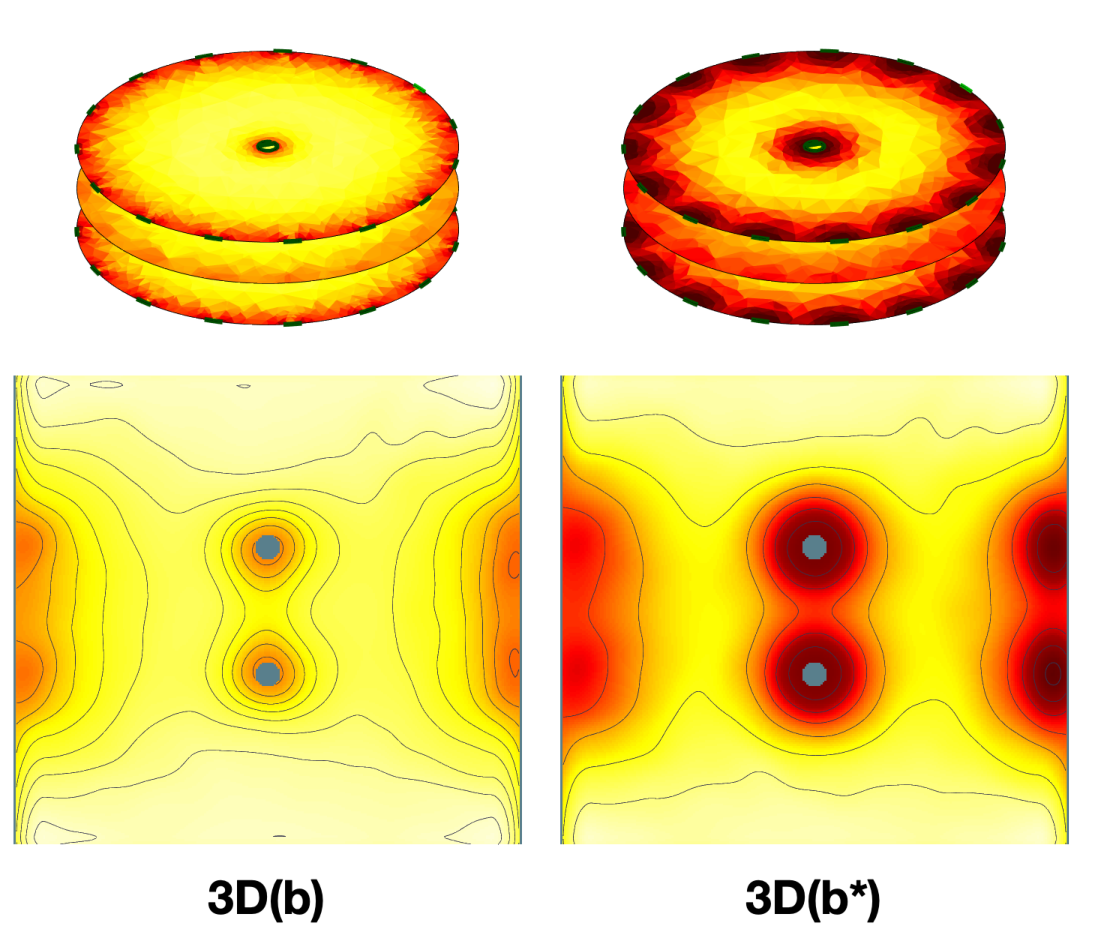
\includegraphics[width=\textwidth]{chapter_5/imgs/Injection_Comparison.pdf}
\caption[Sensitivity using internal electrodes with modified injection patterns]{A comparison between the sensitivity distributions for a typical ``skip 4'' injection pattern pictured on the left (3D(b)) and 
the modified injection and measurement pattern on the right (3D(b*)).}
\label{fig:modified_measurement_sens}
\end{figure}



To quantify image quality, the same object will be reconstructed in multiple situations and is computed as a combination of the following metrics: 
\acrfull{mse} between the reconstructed object and the actual geometry; \acrfull{fwhm} of the reconstructed object; and separability of two identical circular objects in the same reconstruction.


Building on this work simulations will be used to answer more questions on the use of internal electrodes:
\begin{itemize}
\item What internal electrode configuration most improves the internal sensitivity?
\item What is the best injection pattern for measuring activity in the heart region?
\item What is the maximum number of electrodes that can be placed internally while maintaining image quality? 
\item How should internal electrodes be used for current injections?
\item How sensitive is the resulting image to movement of the internal electrodes?
\item In what regions of the FEM is the object reconstruction improved?  
\item Do internal electrodes pose any risk to patient safety?
\end{itemize}

\subsection{Phantom Measurements}
Phantom measurements are used to asses the real-world performance 
of the measurements and configurations 
that were identified in simulations. Two non-conductive circular 
objects are placed and imaged at 4 different separations: 
1 cm, 6 cm, 11 cm and 16 cm 
mid-way between the central probe and the tank wall. 
These separations are used to determine the change 
in resolution between the different configurations. 

In addition to determining the real-world separability the phantom measurements will be used to image a conductive object in a region 
representing the heart region and determine the FWHM and MSE based on the measured location of the object within the phantom dimensions. 
This will be compared to the results obtained through simulations.

\subsection{Animal Data}

Internal electrodes present the opportunity to obtain
a significantly higher sensitivity and with motion correction 
may be used to give a more accurate estimate of arterial pressure.
This paper presents a method of using internal electrodes
while correcting for motion of the internal probe to yield 
high sensitivity near to the esophageal probe.

\section{Methods}
The forward model was constructed using EIDORS version 
3.10~\cite{Adler2019} using \verb!mk_library_model!~\cite{Grychtol2012} 
the internal electrode was added
as an extra structure. This model was also used
to identify the heart and lung regions.
The sensitivity of the lamb model was calculated from 
the Jacobian using 
the method from~\cite{Stowe2020}.
Sensitivity profiles using 32 electrodes with
and without 4 internal electrodes
are shown in fig. \ref{fig:sens_example}.

Data were collected in 3 ewes during ventilation 
under general anesthetic using the
SenTec EIT Pioneer Set.
30 second recordings were
made during regular ventilation with a volume of 
400 \pm 50 ml, frequency of 0.2 \pm 0.05 Hz, and peep of 6.
Recordings were repeated for several 
ventilation scenarios including: high volume (+100 ml),
low volume (-100 ml), 
high frequency (+0.17 Hz), 
low frequency (0.07 Hz), 
high peep (10) and low peep (4). 

All breaths in each 30 second segment were 
ensemble averaged to 
give one representative breath for each scenario.
\begin{figure}[H]
\centering
% Use the following line with your images (pdf preferred)
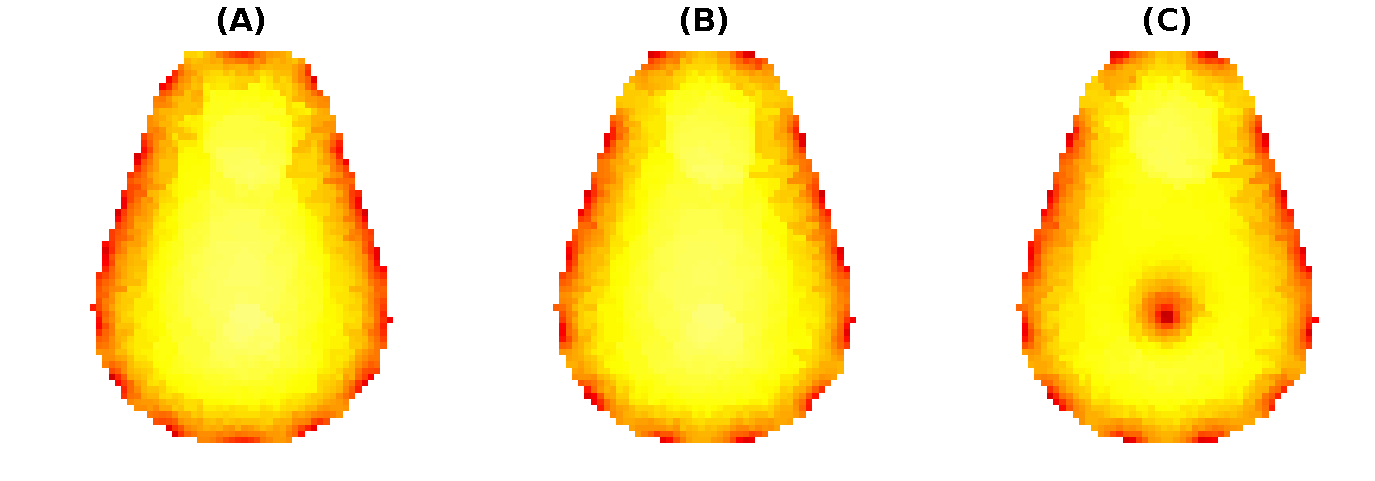
\includegraphics[width=.96\columnwidth]{chapter_5/imgs/lamb_sensitivity_profiles.pdf}
\caption[Sensitivity distribution in a lamb model]{\label{fig:sens_example}%
Sensitivity distribution averaged across 10 evenly spaced layers
between the electrode planes in the lamb model for: 
A) 32 external electrodes 
B) 28 external electrodes 
c) 28 external electrodes and 4 internal electrodes
}
\label{fig:sens_example}
\end{figure}

Images of one averaged breath per recording
were reconstructed using the 3D GREIT 
algorithm~\cite{bartek2016} which minimizes the effect
of electrode motion on the resulting image.
Results were compared for both 
external only and internal electrode configurations
using the same recording.
To obtain results with only external electrodes  all 
injections and measurements using internal electrodes 
were removed prior to reconstruction. 
Measurements on injecting electrodes were always removed.
Images from subject 3 during regular ventilation are 
shown  below in fig.~\ref{fig:img_example}.
With internal electrodes impedance changes at the cardiac frequency had a magnitude of 6.4\% \pm 4.35\%
of the ventilation frequency and without internal electrodes the amplitude of the cardiac frequency
was 0.8\% \pm 0.3\% of the ventilation frequency signal.
\begin{figure}[H]
\centering
% Use the following line with your images (pdf preferred)
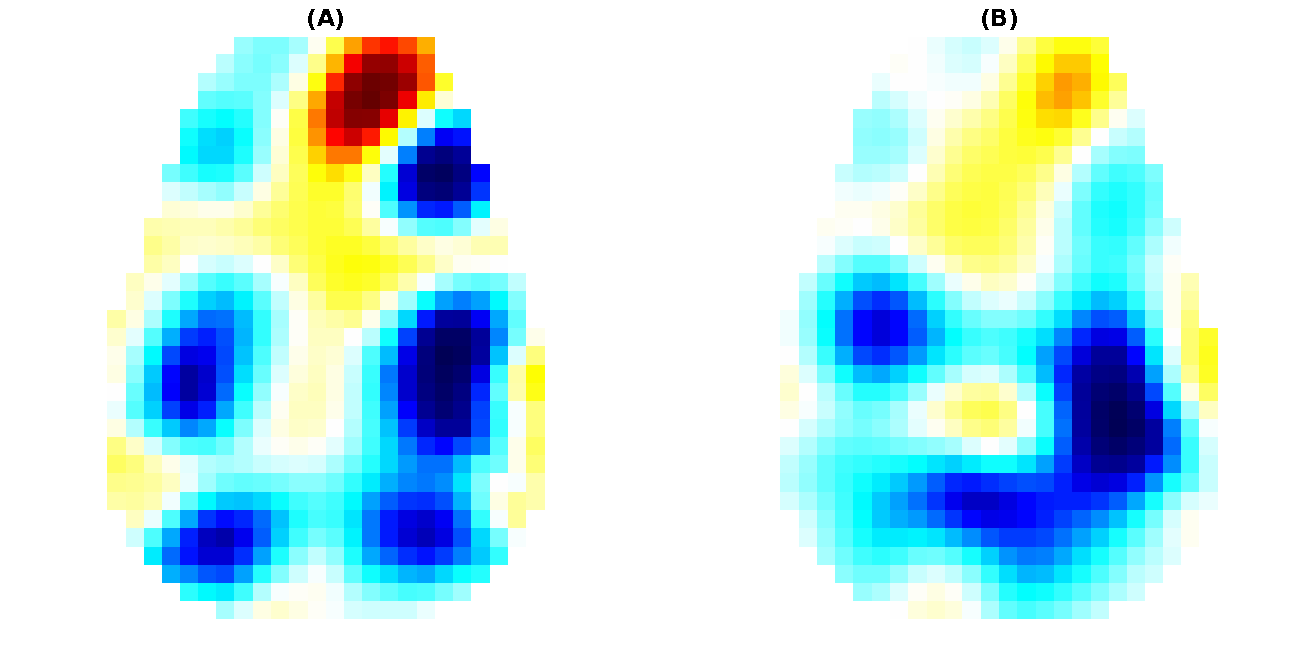
\includegraphics[width=.96\columnwidth]{chapter_5/imgs/lamb_imgs.pdf}
\caption[Reconstructed image of a single breath]{\label{fig:img_example}%
A single breath imaged with:
A) no current injections or measurements on internal
electrodes 
b) with internal electrodes
}
\label{fig:img_example}
\end{figure}
\section{Conclusions}
Reconstructions using the GREIT algorithm
with internal electrodes on 
an esophageal probe were able to give increased
sensitivity to cardiac-frequency impedance changes 
and may allow for better measures of blood pressure and pulse
wave velocity.   



